\documentclass[main.tex]{subfiles} 
\begin{document}

\newpage
\section*{Resultater \& Drøfting}
\label{sec:4}

Når elever skal vurderes så kan dette gjøres på flere måter:
\begin{itemize}
\item Normalfordeling og fast poengsum : da blir vurderingsgrunnlaget \emph{de andre elevenes prestasjoner}. 
Dette blir også referert som relativ vurdering. Vurdering av en individ avhenger da av de andre
elevenes prestasjoner. Ved fast poengsum innebærer det at det er etter poeng oppnåelse elevene blir vurdert. 
Da vil karakterene avgjøres ut ifra hvor mye peongsum eleven har klart å oppnå. Her vil ofte vanskelig oppgaver
bli vektlagt mer enn enkelere oppgaver.
\item Individrelatert kriterier : da vurderes eleven utelukkende i forhold til sine egne forutsetninger
og tidligere prestasjoner. I grunnskolen skal vurderingen uten karakterer i hovedsak være 
individrelatert  (\citeNP[s. 25]{hell07}).
\item Målrelatert kriterier : kvalitetsstandarden blir da en didaktisk kontretisering av kompetansemål.
 I grunnskolen skal vurderingen med karakterer skje etter målrelaterte kriterier (\citeNP[s. 26]{hell07}).
\item Kompetansemål : da vurderes elevene utfra hvilket nivå eller trinn (i henhold til Bloom's taksonomi) 
                      de demonstrer i sin oppnåelse av kompetansemålene.
\end{itemize}
Jeg er nok enig i at bruken av individrelatert vurdering er en god vurderingsgrunnlag i situasjoner
der karakterer ikke brukes. Denne vurderingsformen oppfyller kriterier for god vurdering,
siden den brukes til å fortelle eleven hvor hen befinner seg i sitt studieløp/progresjon.
Når lærer og elev sammen setter individuelle mål, både nærliggende og langsikte, da vil eleven
gjennom et slikt vurderingsgrunnlag få konkete tilbakemeldinger og fremovermeldinger som 
fokuserer på nettopp elevens prestasjoner og målsettinger som hen har laget sammen med
læreren. Det kan også være fordelsaktig å koble målsettingene til kompetansenivå eleven demonstrerer
og jobbe mot høyre kompetansenivå. For eksempel diskutere er et høyt kompetansenivå, der eleven 
kan trekke sammnenhenger og redegjøre for sine tanker om en problemstilling. I motsetning er
å beskrive et middels kompetansenivå (i Bloom's taksonomi).

Siden min hensikt var å kartlegge elevenes svakheter, da er det passende å isteden bruke individrelaterte kritier 
og koble inn kompetansemålene. Til en kartleggingsprøve så er det vanskelig å trekke inn individrelaterte kriterier
med mindre lærer har godt kjennskap til eleven på forhånd. Jeg koblet dessverre ikke inn kompetansemålene heller, 
noe som det bør brukes mer av. Gjennom noen av mine samtaler med elever, oppdaget jeg fort at det var få som trakk 
forbindelsen mellom egen læring og koblingen til kompetansemålene. For undervisere regnes det som en god praksis at 
elevene er alltid bevisste om hvorfor de lærer det de lærer og hvor de er på vei. \citeA[s. 136]{klet13} beskriver 
en god undervisningsseksens der lærere klarer å balansere mellom tilegnelses-, utprøvings-, og 
konsolideringssituasjoner. Ifølge Klette har norske klasserom ensidige tendenser i bruken av varierte arbeidsmåter. 
Slik det kan ses fra figur \ref{fig:odeg10}, er det for eksempel lite konsolideringssituasjoner. Lærernes 
metalæringsaktiviteter regnes som særlig avgjørende for å sikre elevenes læring (\citeNP[s. 186]{klet13}). Å bruke 
dette som et fast organiserende prinsipp, blir derimot sjelden gjennomført (\citeNP[s. 26]{odeg10}).
\begin{figure}[h!]
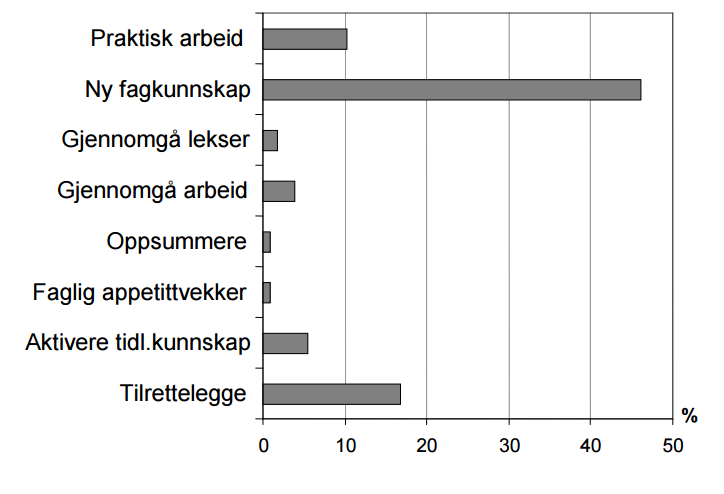
\includegraphics[scale = 0.6]{../figures/undervisnings_aktivitet.png}
\caption{Oversikt over naturfaglærernes undervisningstilbud til elevene fra PISA+ studie. Kilde: 
\protect\citeA{odeg10}.}
\label{fig:odeg10}
\end{figure}

Før resultatene til kartleggingsprøven var jeg informert av min veileder om at klassens snitt lå et sted mellom
karakter 2 og 3. Dermed forventet jeg også at elevene ville prestere lavt på kartleggingsprøven. På figur 
\ref{fig:scoreoversikt} kan vi se at mange elever ligger under en score på 4 :
\begin{figure}[h!]
\centering
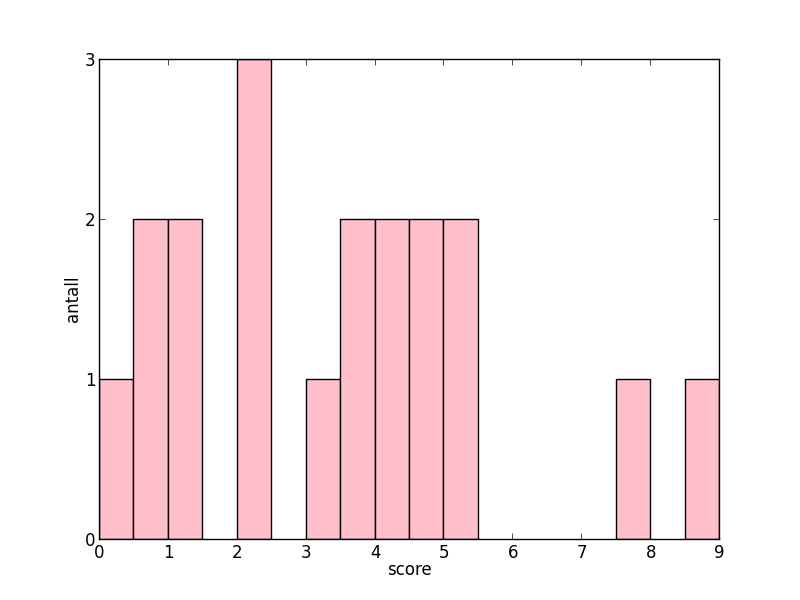
\includegraphics[scale = 0.5]{../figures/scoreoversikt.png}
\caption{Resultater fra kartleggingsprøven - Oversikt over score}
\label{fig:scoreoversikt}
\end{figure}

Siden jeg hadde valgt å ikke gi elevene enn slutt vurdering, annet enn en poengsum hadde det dessverre en negativ 
effekt. Elevene anstrengte ikke like hardt til testen som de ellers ville ha gjort hvis testen var en prøve.
 Jeg hadde dessuten vektlagt de ``vanskelige'' oppgavene mye mer enn de 
``enkle''. Nesten alle elever på tvers av nivå og ferdigheter hadde 
problemmer med å løse disse oppgavene og veldig få klarte å gå over en score på 5 ut av 10. Dermed fikk jeg ikke 
veldig mye informasjon om elevene gjennom poengsum. Ofte var det de over middelssterke elevene i klassen som tangerte
mot 5 i poengsum. Kun en elev klarte å oppnå en score på 8.5, hvor den eneste ``feilen'' eleven gjorde var å
feiltolke oppgave 4.b (dette blir diskutert i neste seksjon). Siden eleven demonstrerte så pass sterke ferdigheter 
burde det kanskje ha vært rom for å gi eleven uttelling for oppfattelsen hen hadde dannet om deloppgaven. 
Uansett konkluderte jeg sammen med veileder at prøven var nok litt vanskeligere enn det burde ha vært. Videre nå vil 
jeg snakke om individuelle oppgaver fra kartleggingsprøven, og diskutere elevenes feiltolninger.
(legg til graf over poengfordeling)

\subsection*{Elevenes feiltolkninger}
Pyskologene Daniel Kahneman og Amos Tversky har satt fram en teoretisk 
ramme for å undersøke læring av sannsynlighet og statistikk. Deres tese er at mennesker uten erfaring, refleksjon og 
innsikt i statistikk, bruker følgende strategier for å bedømme sannsynlighet (\citeNP{udir13}; \citeNP{evan17}):
\begin{itemize}
\item Representativitet : små utvalg skal representere den fordelingen som finnes i populasjonen
\item Tilgjengelighet : sannsynlighet bedømmes ut fra hvor lett det er å huske spesielle tilfeller
\item Resultatorientering : utfallet kan forutses, som ved en deterministisk prosess
\item Konjunksjonsfellen : sannsynligheten for at to hendelser inntreffer samtidig er mindre enn sannsynligheten
for at en av hendelsene inntreffer.
\item Generelt vanskeligheter med betinget sannsynlighet : dvs. vanskeligheter med sannsynligheter hvor et utfall
avhenger av foregående utfall. Imotsetning er utbetinget sannsynlighet utfall der en begivenhet forekommer uavhengig 
av tidligere utfall. 
\end{itemize}
Dette er ofte misoppfattelser som også ligger hos elever med ulike faglig bakgrunn.

Det var en deloppgave i kartleggingsprøven som mange elever feiltolket, og det kan jeg godt
akseptere at oppgaveteksten er lett å tolke på en annen måte :
\par
\begin{figure}[h!]
\centering
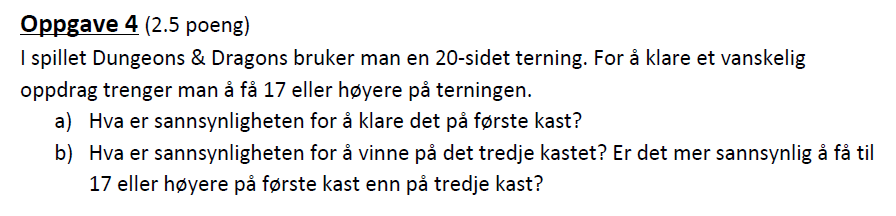
\includegraphics[scale = 0.7]{../figures/oppgave4b.png}
\caption{Oppgave 4}
\label{fig:oppgave4}
\end{figure}
I oppgave b står det \emph{Hva er sannsynligheten for å vinne på det tredje kastet?}. Her var hensikten at
elevene skulle oppfatte det som \emph{Hva er sannsynligheten for å tape på to runder på rad og deretter vinne på 
det tredje kastet?}, men mange oppfattet det som å vinne på tredje kastet uavhengig av hva som forekommer på de 
første to kast. Dermed ville svaret til neste del av deloppgaven, \emph{Er det mer sannsynlig å få til 17 eller 
høyere på første kast enn på det tredje kast?},  være ``like sannsynlig'' og det var ofte det elevene besvarte. 
I oppgave 4.b har elevene anledning til å demonstrere høyt kompetansenivå. Dessverre er formuleringen ikke
godt nok til å trekke elevene inn i et diskurs. Her burde det gjerne ha blitt lagt til en bisetning, som 
for eksempel \emph{``Kan du gi en forklaring?''}. Med slike spørsmål er det lettere å oppdage elevenes
feiltolkninger, fordi da slipper en å få besvarelser som er enten ``ja'' eller ``nei''. Oppgave 
5.b var bedre formulert (se vedlegg 1). Her kreves det eksplisitt en forklaring fra elevene.
Dette er en fin øvelse for elever å demonstrere at de har forstått bruken av utfallstreet. Det var derimot
få elever som fikk til oppgaven, og enda fære som prøvde å gi en forklaring. Etter å snakket med elevene
som forsøkte å løse oppgaven, var forklaringen deres at enten så overså de krav om begrunnelsen, eller de var
ikke sikker på forklaringen. De som overså krav om begrunnelsen, neglisjerte denne delen av oppgaven fordi
de fikk ikke med seg at det skulle legges til en forklaring, og de andre svarte at en forklaring var ikke
viktig å få med. 

\begin{figure}
\centering
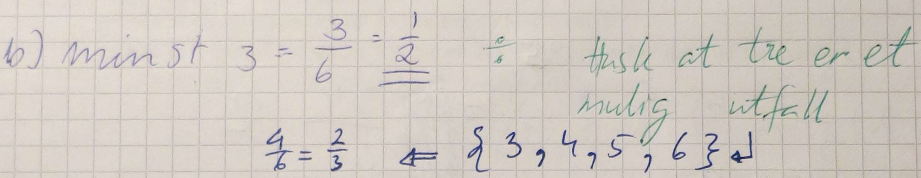
\includegraphics[scale = 0.4]{../figures/maryam.png}
\caption{Oppgave 1}
\label{fig:maryam}
\end{figure}

\begin{figure}
\centering
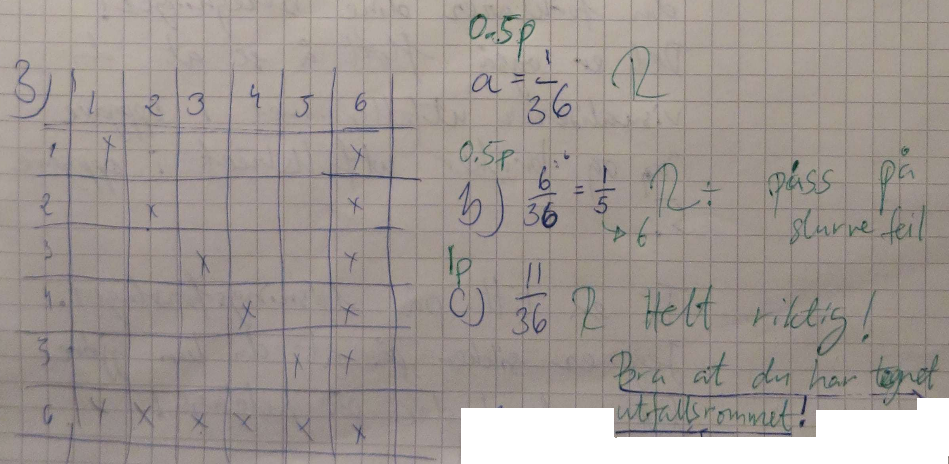
\includegraphics[scale = 0.4]{../figures/maryam2.png}
\caption{Oppgave 3}
\label{fig:maryam2}
\end{figure}

\begin{figure}
\centering
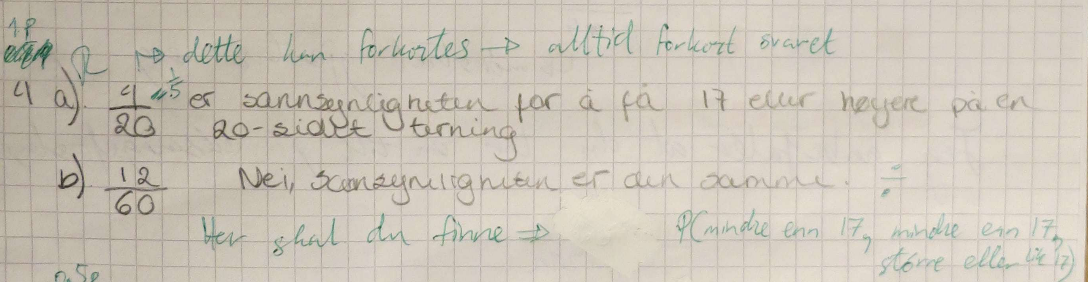
\includegraphics[scale = 0.4]{../figures/maria.png}
\caption{Oppgave 4}
\label{fig:maria}
\end{figure}

\begin{figure}
\centering
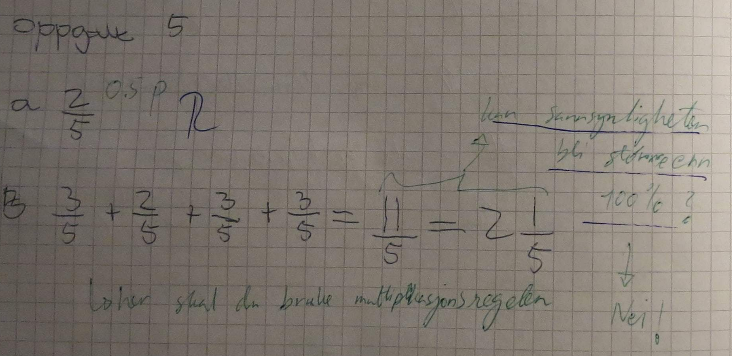
\includegraphics[scale = 0.4]{../figures/mohsin.png}
\caption{Oppgave 5}
\label{fig:mohsin}
\end{figure}


\subsection*{Tilbakemeldinger}

William redegjør for hvorfor tilbakemeldinger noen ganger kan føre til senking 
i elvenes ytelse. Han referer til Kluger og DeNisi (1996), når han summerer opp 
\begin{displayquote}
\textelp{} feedback was least effective when it focused on the task in hand, 
and more effective when it focused on the details at hand, and most effective 
when it focused on the details of the task and involved goal-setting.
(\citeNP[s. 140]{will10})
\end{displayquote}

\begin{figure}
\centering
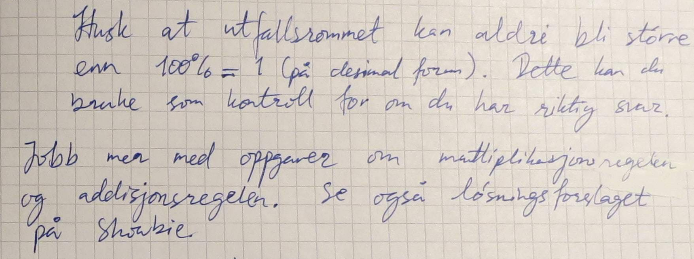
\includegraphics[scale = 0.4]{../figures/mohsin2.png}
\caption{Tilbakemelding og fremovermelding}
\label{fig:mohsin2}
\end{figure}

Et problem som jeg opplevde med kartleggingsprøven var at elever demonstrerte ikke like sterk engasjement
i å besvare riktig. Jeg snakket med en av de sterke elevene som jeg har tidligere observert i timene.
Jeg spurte hen hvorfor hen ikke hadde besvart en spesifikk oppgave og hen svarte med å si at oppgaven 
var lett, men hen ``orket'' ikke å gå gjennom den. Grunnen hen oppga var at siden det ikke var en prøve,
hadde det ikke så mye betyning. Dette samsvarer godt med det \citeA[s. 3]{brbl14} skriver : \emph{Vurdering 
kan ha en betydelig påvirkning på hvordan elever jobber, fordi de oppfatter det som vurderes som det eneste
``som teller''}.


\end{document}
